% ------------------------------------------------------------------------------%%%%%%%%
\section{Theory - \textit{clDice} in Digital Topology}
\label{sec:interp}


In addition to our Theorem 1 in the main paper, %\ref{thm2},
we are providing intuitive interpretations of \textit{clDice} from the digital topology perspective. Betti numbers describe and quantify topological differences in algebraic topology. The first three Betti numbers ($\beta_0$, $\beta_1$, and $\beta_2$) comprehensively capture the manifolds appearing in 2D and 3D topological space. Specifically,
\begin{itemize}[itemsep=-4pt]%leftmargin=*]
    \item $\beta_0$ represents the number of \textit{connected-components},
    \item $\beta_1$ represents the number of \textit{circular holes}%[c.f. Fig. A. \ref{fig_top_ex}]
    , and
    \item $\beta_2$ represents the number of \textit{cavities} %[c.f. Fig. A. \ref{fig_top_ex}] 
    (Only in 3D)
\end{itemize}{}


\begin{figure}[ht!]
\begin{center}

\includegraphics[width=0.13\textwidth]{figs/hole_2d.pdf}
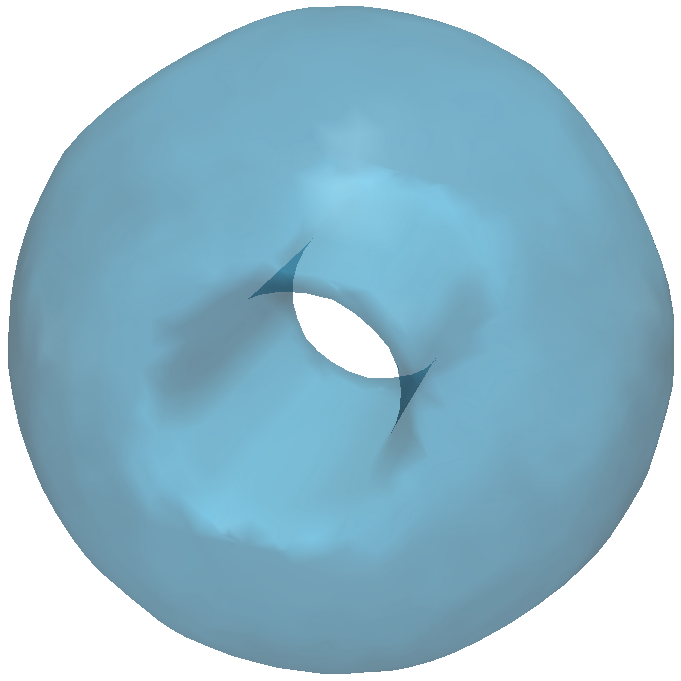
\includegraphics[width=0.14\textwidth]{figs/hole.png}
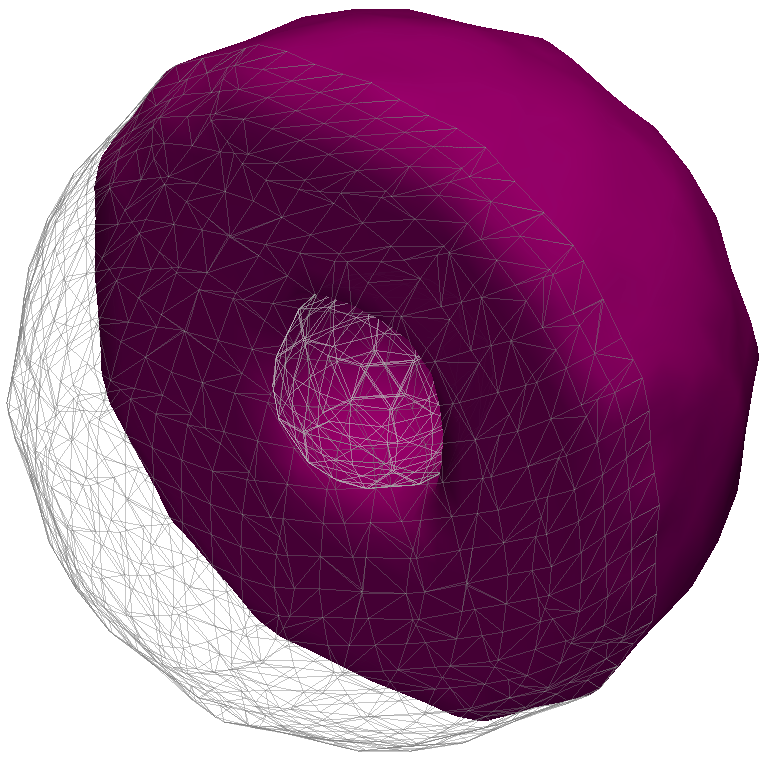
\includegraphics[width=0.14\textwidth]{figs/cavity.png} \\
\end{center}
\caption{Examples of the topology properties. Left, a hole in 2D, in the middle a hole in 3D and right a cavity inside a sphere in 3D.} 
\label{fig_top_ex}
\end{figure}

Using the concepts of Betti numbers and digital topology by Kong et al. \cite{kong1995topology,rosenfeld1979digital}, we formulate the effect of topological changes between a true binary mask ($V_L$) and a predicted binary mask ($V_P$) in Fig. \ref{fig_ghost_miss}. We will use the following definition of \textbf{ghosts} and \textbf{misses}, see Figure \ref{fig_ghost_miss}.


\begin{enumerate}[] %label=\textbf{Top \arabic*},align=left
    \item \textbf{Ghosts in skeleton: } We define ghosts in the predicted skeleton ($S_P$) when $S_P \not\subset V_L$. This means the predicted skeleton is not completely included in the true mask. In other words, there exist false-positives in the prediction, which survive after skeletonization.\label{prop1}
    
    \item \textbf{Misses in skeleton: } We define misses in the predicted skeleton ($S_P$) when $S_L \not\subset V_P$. This means the true skeleton is not completely included in the predicted mask. In other words, there are false-negatives in the prediction, which survive after skeletonization.\label{prop2}
\end{enumerate}



\begin{figure*}[ht!]
\begin{center}

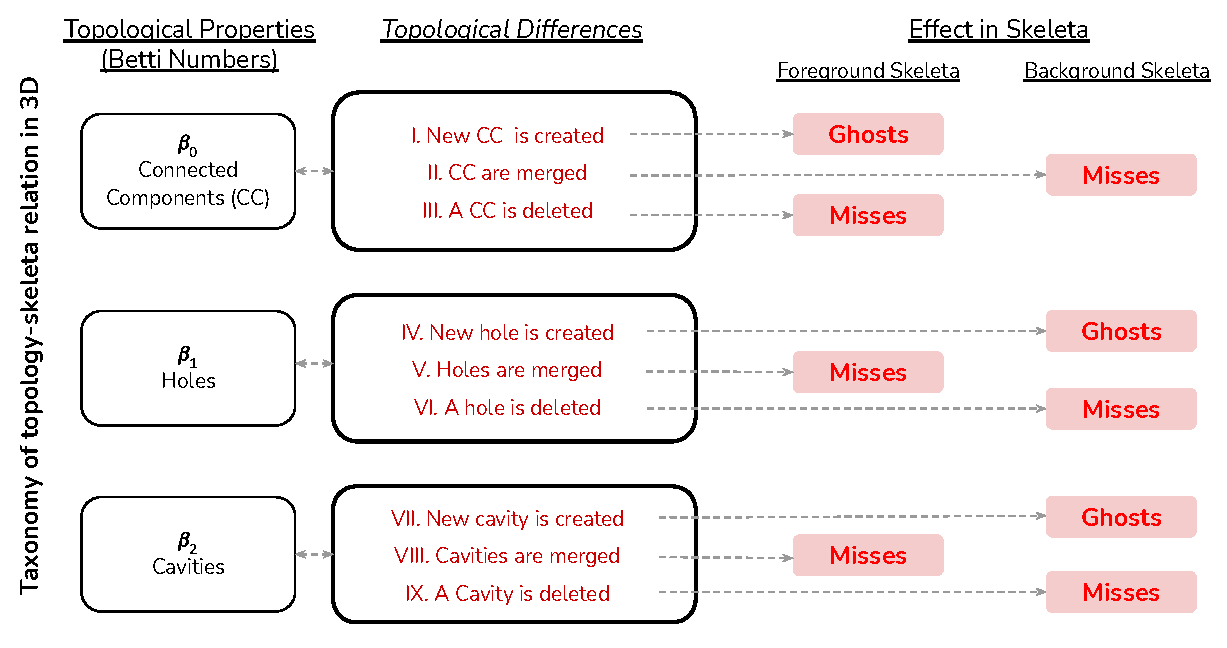
\includegraphics[width=0.95\linewidth]{figs/clDice_CVPR.pdf}
\label{fig_theory}
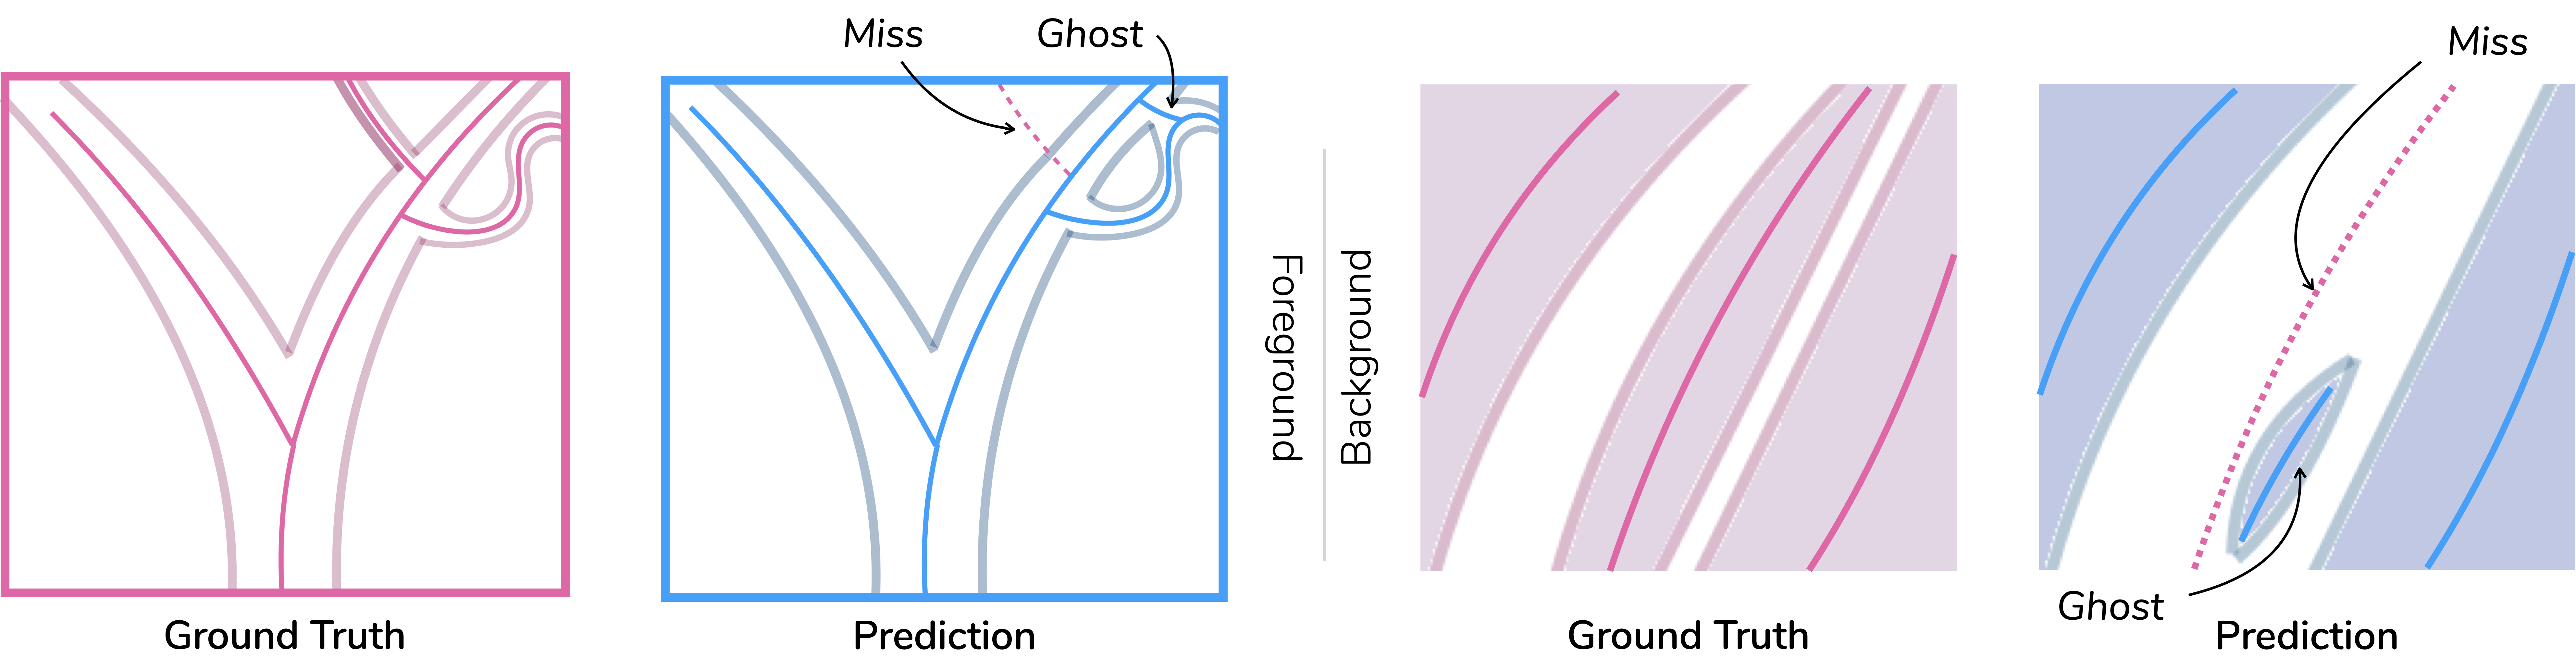
\includegraphics[width=0.92\linewidth]{figs/ghost_miss_cvpr.png}
\end{center}
\caption{Upper part, left, taxonomy of the $iff$ conditions to preserve topology in 3D using the concept of Betti numbers \cite{kong1995topology,kong1989digital}; interpreted as the necessary violation of skeleton properties for any possible topological change in the terminology of ghosts and misses (upper part right) . Lower part, intuitive depictions of ghosts and misses in the prediction; for the skeleton of the foreground (left) and the skeleton of the background (right).}
\label{fig_ghost_miss}
\end{figure*}

The false positives and false negatives are denoted by $V_P\setminus V_L$ and $V_L\setminus V_P$, respectively, where $\setminus$ denotes a set difference operation. The loss function aims to minimize both errors. We call an error correction to happen when the value of a previously false-negative or false-positive voxel flips to a correct value. Commonly used voxel-wise loss functions, such as Dice-loss, treat every false-positive and false-negative equally, irrespective of the improvement in regards to topological differences upon their individual error correction. Thus, they cannot guarantee homotopy equivalence until and unless every single voxel is correctly classified. In stark contrast, we show in the following proposition that \textit{clDice} guarantees homotopy equivalence under \textit{a minimum error correction.}


% \noindent 
\begin{proposition}

For any topological differences between $V_P$ and $V_L$, achieving optimal \textit{clDice} to guarantee homotopy equivalence requires a minimum error correction of $V_P$.
\end{proposition}

\begin{proof}
From Fig \ref{fig_ghost_miss}, any topological differences between $V_P$ and $V_L$ will result in ghosts or misses in the foreground or background skeleton. Therefore, removing ghosts and misses are sufficient conditions to remove topological differences. Without the loss of generalizability, we consider the case of ghosts and misses separately:\\

For a \textbf{ghost} $g \subset S_P, \exists \mbox{ a set of predicted voxels } E1 \subset \{V_P \setminus V_L\}\mbox{ such that } V_P \setminus E
1$ does not create any misses and removes $g$. Without the loss of generalizability, let's assume that there is only one ghost $g$. Now, to remove $g$, under a minimum error correction of $V_P$, we have to minimize $|E1|$. Let's say an optimum solution $E1_{min}$ exists. By construction, this implies that $V_P\setminus E1_{min}$ removes $g$.


For a \textbf{miss} $m \subset V_P^\complement, \exists \mbox{ a set of predicted voxels } E2 \subset \{V_L \setminus V_P\}\mbox{ such that } V_P \cup E2$ does not create any ghosts and removes $m$. Without the loss of generalizability, let's assume that there is only one miss $m$. Now, to remove $m$, under a minimum error correction of $V_P$, we have to minimize $|E2|$. Let's say an optimum solution $E2_{min}$ exists. By construction, this implies that $V_P\cup E2_{min}$ removes $m$.\\

Thus, in the absence of any ghosts and misses, from Lemma \ref{obs1}, \textit{clDice}=1 for both foreground and background. Finally, Therefore, Theorem 1 (from the main paper) guarantees homotopy equivalence.
\end{proof}


\begin{restatable}[]{lemma}{obsone}
\label{obs1}
In the absence of any ghosts and misses \textit{clDice}=1.
\end{restatable}

\begin{proof}
The absence of any ghosts $S_P \in V_L$ implies $Tprec=1$; and the absence of any misses $S_L \in V_P$ implies $Tsens=1$. Hence, \textit{clDice}=1.
\end{proof}

\subsection{Interpretation of the Adaption to Highly Unbalanced Data According to Digital Topology:}
Considering the adaptions we described in the main text, the following provides analysis on how these assumptions and adaptions are funded in the concept of ghosts and misses, described in the previous proofs. Importantly, the described adaptions are not detrimental to the performance of \textit{clDice} for our datasets.
We attribute this to the non-applicability of the necessary conditions specific to the background (i.e. II, IV, VI, VII, and IX in Figure \ref{fig_theory}), as explained below: 

\begin{itemize}[,itemsep=-2pt]
    \item II. $\rightarrow$ In tubular structures, all foreground objects are eccentric (or anisotropic). Therefore isotropic skeletonization will highly likely produce a ghost in the foreground.
    \item IV. $\rightarrow$ Creating a hole outside the labeled mask means adding a ghost in the foreground. Creating a hole inside the labeled mask is extremely unlikely because no such holes exist in our training data.
    \item VI. $\rightarrow$ The deletion of a hole without creating a miss is extremely unlikely because of the sparsity of the data.
    \item VII.and IX. (only for 3D) $\rightarrow$ Creating or removing a cavity is very unlikely because no cavities exist in our training data.
    %\item IX. (only for 3D) $\rightarrow$ Cavities do not exist in the real dataset.
\end{itemize}

\section{Additional Qualitative Results} 
\begin{figure*}[]
\label{supp_road}
\centering

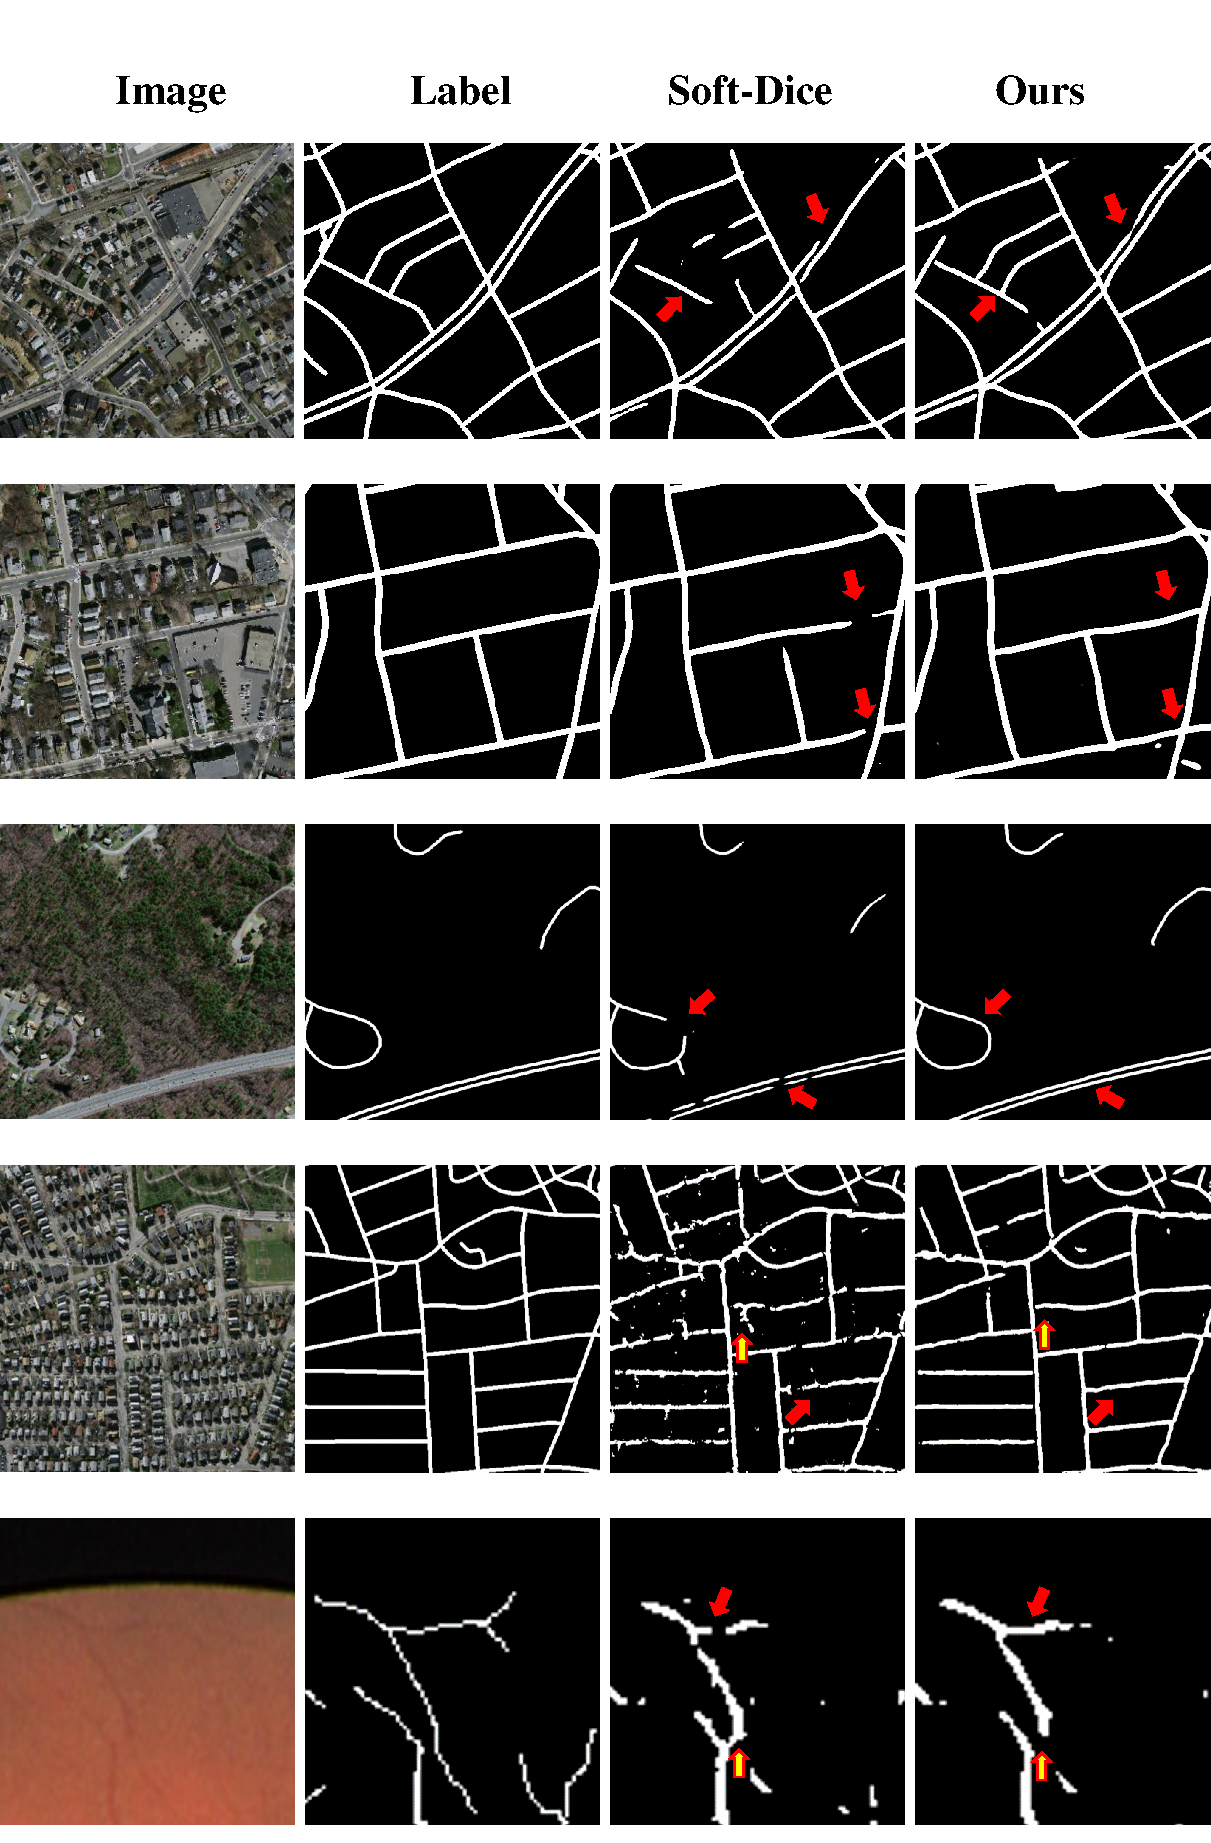
\includegraphics[width=0.78\linewidth]{figs/suppl/Appendix_clDice_qualitative_results.pdf}

\caption{\footnotesize Qualitative results:  for the Massachusetts Road dataset and  for the DRIVE retina dataset (last row). From left to right, the real image, the label, the prediction using soft-dice and the predictions using the proposed $\mathcal{L}_c (\alpha=0.5)$, respectively. The first three rows are U-Net results and the fourth row is an FCN result. This indicates that \textit{soft-clDice} segments road connections which the soft-dice loss misses. Some,  but  not  all,  missed  connections  are  indicated with solid red arrows, false positives are indicated with red-yellow arrows.}
\end{figure*}


\begin{figure*}[]
\label{supp_3d}
\centering

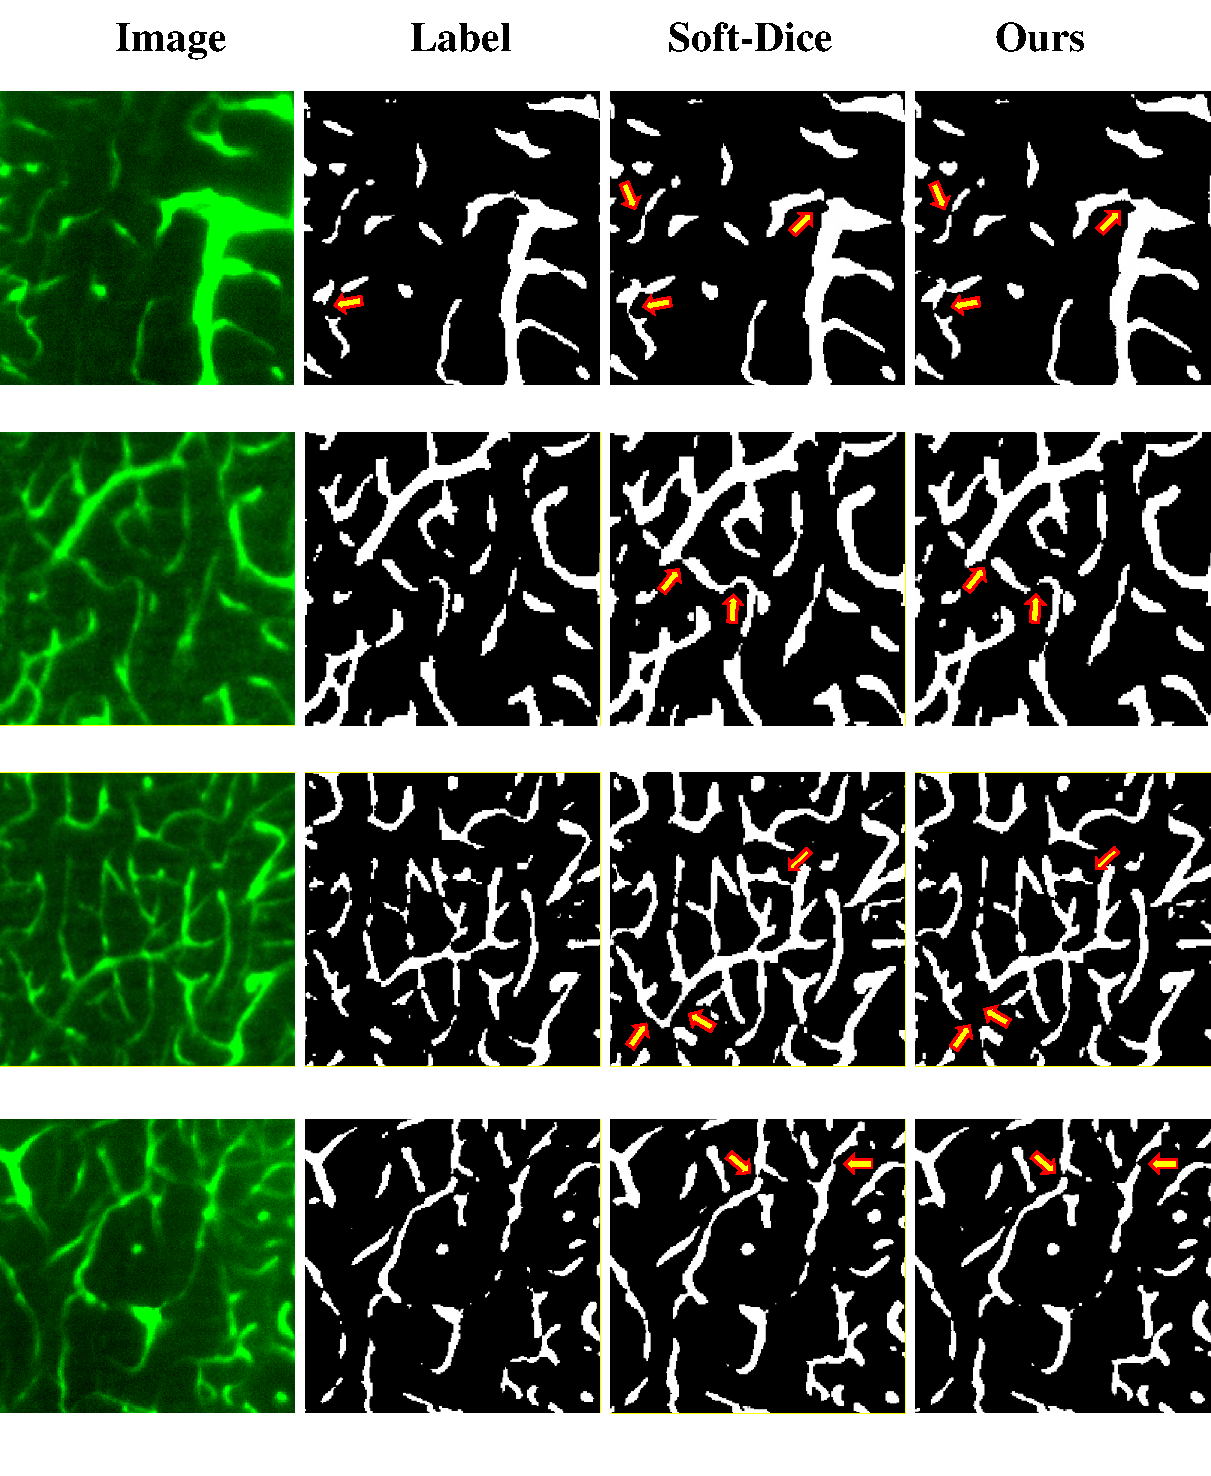
\includegraphics[width=0.78\linewidth]{figs/suppl/Appendix_3D_clDice_qualitative_results.pdf}
\caption{\footnotesize Qualitative results: 2D slices of the 3D vessel dataset for different sized field of views. From left to right, the real image, the label, the prediction using soft-dice and the U-Net predictions using $\mathcal{L}_c (\alpha=0.4)$, respectively. These images show that \textit{soft-clDice} helps to better segment the vessel connections. Importantly the networks trained using soft-dice over-segment the vessel radius and segments incorrect connections. Both of these errors are not present when we train including \textit{soft-clDice} in the loss. Some,  but  not  all, false positive connections are indicated with red-yellow arrows.
}
\end{figure*}

\section{Comparison to Other Literature:} 

A recent pre-print proposed a region-separation approach, which aims to tackle the issue by analysing disconnected foreground elements \cite{oner2020promoting}. Starting with the predicted distance map, a network learns to close ambiguous gaps by referring to a ground truth map which is dilated by a five-pixel kernel, which is used to cover the ambiguity. However, this does not generalize to scenarios with a close or highly varying proximity of the foreground elements (as is the case for e.g. capillary vessels, synaptic gaps or irregular road intersections). Any two foreground objects which are placed at a twice-of-kernel-size distance or closer to each other will potentially be connected by the trained network. This is facilitated by the loss function considering the gap as a foreground due to performing dilation in the training stage. Generalizing their approach to smaller kernels has been described as infeasible in their paper \cite{oner2020promoting}.

\section{Datasets and Training Routine}

For the DRIVE vessel segmentation dataset, we perform three-fold cross-validation with 30 images and deploy the best performing model on the test set with 10 images. For the Massachusetts Roads dataset, we choose a subset of  120 images (ignoring imaged without a network of roads) for three-fold cross-validation and test the models on the 13 official test images.  For CREMI, we perform three-fold cross-validation on 324 images and test on 51 images. For the 3D synthetic dataset. we perform experiments using 15 volumes for training, 2 for validation, and 5 for testing.
For the Vessap dataset, we use 11 volumes for training, 2 for validation and 4 for testing. In each of these cases, we report the performance of the model with the highest clDice score on the validation set.


\section{Network Architectures} 
We use the following notation: $In(input~channels)$, $Out(output~channels)$, \\ $B(output~channels)$ present input, output, and bottleneck information(for U-Net); $C(filter~size, output~channels)$ denote a convolutional layer followed by $ReLU$ and batch-normalization; $U(filter~size, output~channels)$ denote a trans-posed convolutional layer followed by $ReLU$ and batch-normalization; $\downarrow 2$ denotes maxpooling; $\oplus$ indicates concatenation of information from an encoder block. We had to choose a different FCN architecture for the Massachusetts road dataset because we realize that a larger model is needed to learn useful features for this complex task.

\subsection{Drive Dataset}
\subsubsection{FCN :}
$IN(\mbox{3 ch})\rightarrow C(3,5)\rightarrow C(5,10) \rightarrow C(5,20)\rightarrow C(3,50)\rightarrow C(1,1)\rightarrow Out(1)$
\subsubsection{Unet :}
\paragraph{ConvBlock :} $C_B(3, out~size)\equiv C(3,out~size)\rightarrow C(3,out~size)\rightarrow \downarrow 2$
\paragraph{UpConvBlock:} $U_B(3, out~size)\equiv U(3,out~size)\rightarrow \oplus\rightarrow C(3,out~size)$
\paragraph{Encoder :}
$IN(\mbox{3 ch})\rightarrow C_B(3,64)\rightarrow C_B(3,128) \rightarrow C_B(3,256)\rightarrow C_B(3,512)\rightarrow C_B(3,1024)\rightarrow B(1024)$
\paragraph{Decoder :}
$B(1024)\rightarrow U_B(3,1024)\rightarrow U_B(3,512)\rightarrow U_B(3,256) \rightarrow U_B(3,128)\rightarrow U_B(3,64)\rightarrow Out(1)$

\subsection{Road Dataset}
\subsubsection{FCN :}
$IN(\mbox{3 ch})\rightarrow C(3,10)\rightarrow C(5,20)\rightarrow C(7,30)\rightarrow C(11,30)\rightarrow C(7,40) \rightarrow C(5,50)\rightarrow C(3,60)\rightarrow C(1,1)\rightarrow Out(1)$
\subsubsection{Unet :}
Same as Drive Dataset, except we used 2x2 up-convolutions instead of bilinear up-sampling followed by a 2D-convolution with kernel size 1.

\subsection{Cremi Dataset}
% \subsubsection{FCN :}
% Same as Road Dataset.
\subsubsection{Unet :}
Same as Road Dataset. 

\subsection{3D Dataset }
\subsubsection{3D FCN :}
$IN(\mbox{1 or 2 ch})\rightarrow C(3,5)\rightarrow C(5,10) \rightarrow C(5,20)\rightarrow C(3,50)\rightarrow C(1,1)\rightarrow Out(1)$
\subsubsection{3D Unet :}
\paragraph{ConvBlock :} $C_B(3, out~size)\equiv C(3,out~size)\rightarrow C(3,out~size)\rightarrow \downarrow 2$
\paragraph{UpConvBlock:} $U_B(3, out~size)\equiv U(3,out~size)\rightarrow \oplus\rightarrow C(3,out~size)$
\paragraph{Encoder :}
$IN(\mbox{1 or 2 ch})\rightarrow C_B(3,32)\rightarrow C_B(3,64) \rightarrow C_B(3,128)\rightarrow C_B(5,256)\rightarrow C_B(5,512)\rightarrow B(512)$
\paragraph{Decoder :}
$B(512)\rightarrow U_B(3,512) \rightarrow U_B(3,256)\rightarrow U_B(3,128) \rightarrow U_B(3,64)\rightarrow U_B(3,32)\rightarrow Out(1)$


\begin{table}[ht!]
\centering
\caption{Total number of parameters for each of the architectures used in our experiment.}
\begin{tabular}{ccc}
\hline
Dataset & Network & Number of parameters \\
\hline
\hline
Drive   & FCN     & 15.52K               \\
        & UNet    & 28.94M               \\
        \hline
Road    & FCN      & 279.67K              \\
\hline
Cremi    & UNet      & 31.03M              \\
\hline
3D      & FCN 2ch    & 58.66K               \\
        & Unet 2ch    & 19.21M             \\
\hline
\end{tabular}
\end{table}
%\clearpage





\section{Soft Skeletonization Algorithm}

\begin{figure}[ht!]
\centering
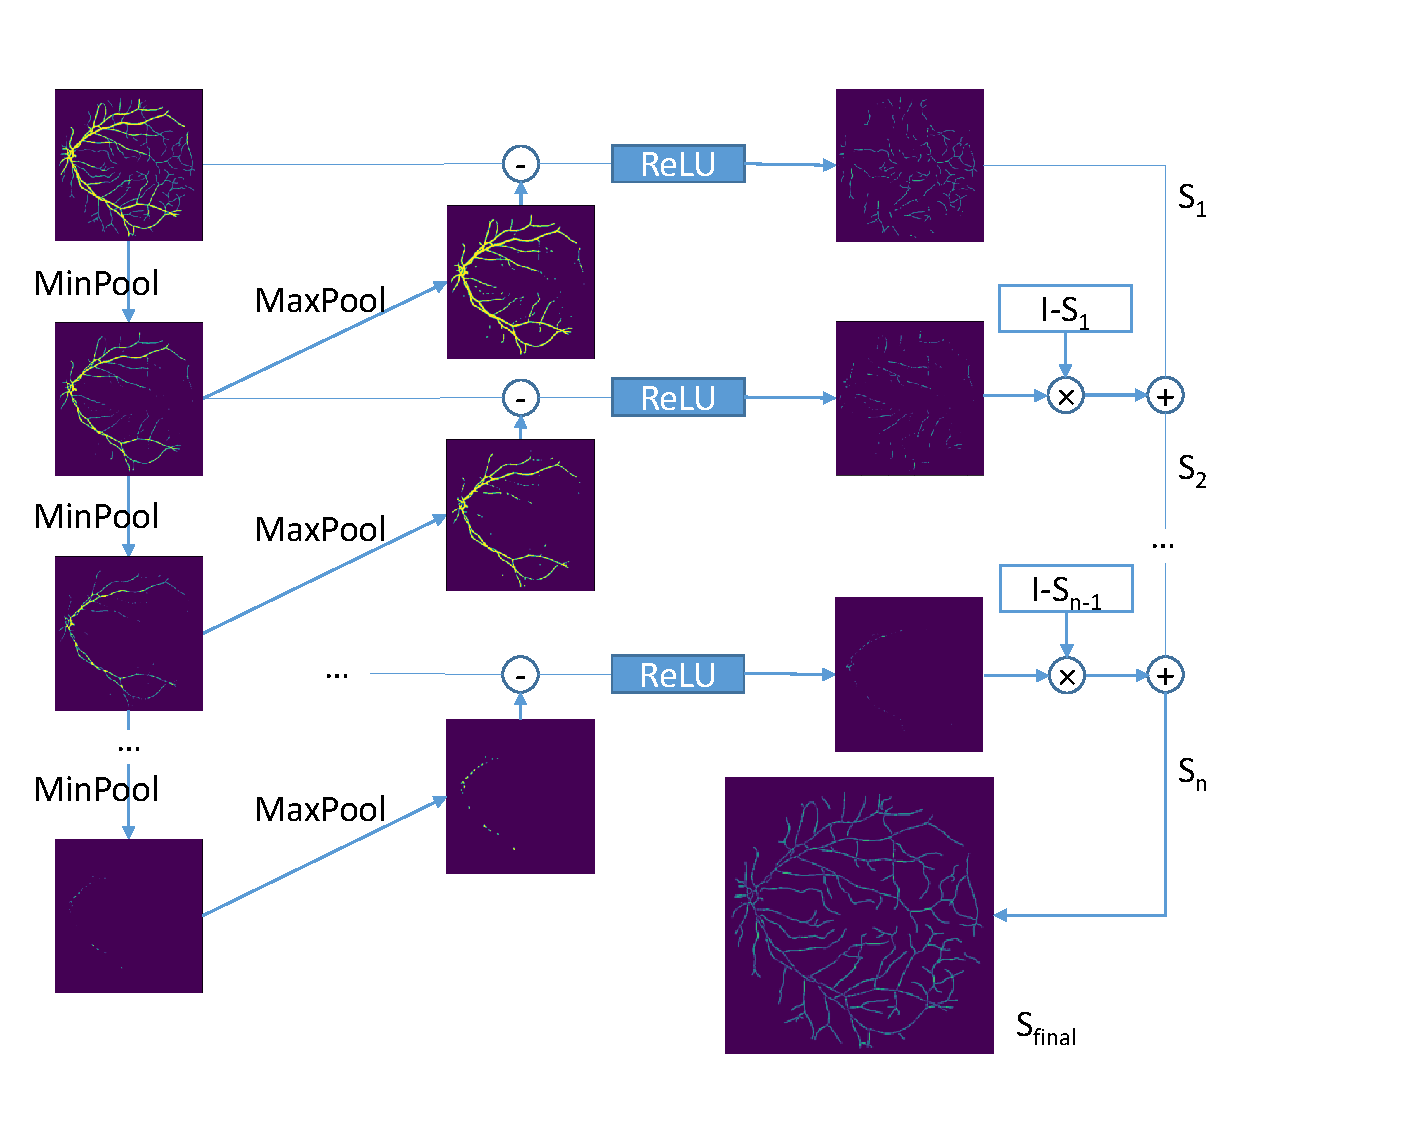
\includegraphics[width=1\linewidth]{figs/suppl/skel_grafik.pdf}

\caption{Scheme of our proposed differentiable skeletonization. On the top left the mask input is fed. Next, the input is reatedly eroded and dilated. The resulting erosions and dilations are compared to the image before dilation. The difference between thise images is part of the skeleton and will be added iteratively to obtain a full skeletonization. The ReLu operation eliminates pixels that were generated by the dilation but are not part of the oirginal or eroded image.}
\label{example_skel}
\end{figure}



\section{Code for the \textit{clDice} similarity measure and the \textit{soft-clDice} loss (PyTorch):}


\subsection{\textit{clDice} measure}
\footnotesize
\begin{lstlisting}[language=Python]
from skimage.morphology import skeletonize
import numpy as np
def cl_score(v, s):
    return np.sum(v*s)/np.sum(s)
def clDice(v_p, v_l):
    tprec = cl_score(v_p,skeletonize(v_l))
    tsens = cl_score(v_l,skeletonize(v_p))
    return 2*tprec*tsens/(tprec+tsens)
\end{lstlisting}

\subsection{\textit{soft-skeletonization} in 2D}
\begin{lstlisting}[language=Python]
import torch.nn.functional as F
def soft_erode(img):
    p1 = -F.max_pool2d(-img, (3,1), (1,1), (1,0))
    p2 = -F.max_pool2d(-img, (1,3), (1,1), (0,1))
    return torch.min(p1,p2)

def soft_dilate(img):
    return F.max_pool2d(img, (3,3), (1,1), (1,1))

def soft_open(img):
    return soft_dilate(soft_erode(img))
    
def soft_skel(img, iter):
    img1 = soft_open(img)
    skel = F.relu(img-img1)
    for j in range(iter):
        img = soft_erode(img)
        img1 = soft_open(img)
        delta = F.relu(img-img1)
        skel = skel + F.relu(delta-skel*delta)
    return skel
\end{lstlisting}

\subsection{\textit{soft-skeletonization} in 3D}
\begin{lstlisting}[language=Python]
import torch.nn.functional as F

def soft_erode(img):
    p1 = -F.max_pool3d(-img,(3,1,1),(1,1,1),(1,0,0))
    p2 = -F.max_pool3d(-img,(1,3,1),(1,1,1),(0,1,0))
    p3 = -F.max_pool3d(-img,(1,1,3),(1,1,1),(0,0,1))

    return torch.min(torch.min(p1, p2), p3)

def soft_dilate(img):
    return F.max_pool3d(img,(3,3,3),(1,1,1),(1,1,1))

def soft_open(img):
    return soft_dilate(soft_erode(img))

def soft_skel(img, iter_):
    img1  =  soft_open(img)
    skel  =  F.relu(img-img1)
    for j in range(iter_):
        img  =  soft_erode(img)
        img1  =  soft_open(img)
        delta  =  F.relu(img-img1)
        skel  =  skel +  F.relu(delta-skel*delta)
    return skel

\end{lstlisting}
\normalsize


\section{Evaluation Metrics}
\noindent As discused in the text, we compare the performance of various experimental setups using three types of metrics: volumetric, graph-based and topology-based. 


\subsection{ Overlap-based:}
Dice coefficient, Accuracy and \textit{clDice}, we calculate these scores on the whole 2D/3D volumes. \textit{clDice} is calculated using a morphological skeleton (skeletonize3D from the skimage library). 

\subsection{Graph-based:} We extract graphs 
from random patches of $64\times64$ pixels in 2D and $48\times48\times48$ in 3D images.  

For the StreetmoverDistance (SMD) \cite{belli2019image} we uniformly sample a fixed number of points from the graph of the prediction and label, match them and calculate the Wasserstein-distance between these graphs. 
For the junction-based metric (Opt-J) we compute the F1 score of junction-based metrics, recently proposed by \cite{citrarotowards}. According to their paper this metric is advantageous over all previous junction-based metrics as it can account for nodes with an arbitrary number of incident edges, making this metric more sensitive to endpoints and missed connections in predicted networks. For more information please refor to their paper. 


\subsection{Topology-based:} 
For topology-based scores we calculate the Betti Errors for the Betti Numbers $\beta_0$ and $\beta_1$. Also, we calculate the Euler characteristic, $\chi = V-E+F$, where $E$ is the number of edges, $F$ is the number of faces and $V$ is the number of vertices. We report the relative Euler characteristic error ($\chi_{ratio}$), as the ratio of the $\chi$ of the predicted mask and that of the ground truth. Note that a $\chi_{ratio}$ closer to one is preferred. All three topology-based scores are calculated on random patches of $64\times64$ pixels in 2D and $48\times48\times48$ in 3D images. 




\section{Additional Quantitative Results}

\begin{table}[ht!]

\caption{ Quantitative experimental results for the 3D synthetic vessel dataset. Bold numbers indicate the best performance. We trained baseline models of binary-cross-entropy (BCE), softDice and mean-squared-error loss (MSE) and combined them with our \textit{soft-clDice} and varied the $\alpha > 0$. For all experiments we observe that using \textit{soft-clDice} in $\mathcal{L}_{c}$ results in improved scores  compared to \emph{soft-Dice}. This improvement holds for almost $\alpha > 0$. We observe that \textit{soft-clDice} can be efficiently combined with all three frequently used loss functions.}

\centering
\label{synth_data_table}

\begin{tabular}{|p{2.2cm}|p{1.4cm}|p{1.4cm}|}
        \hline
        Loss&Dice&clDice\\
        \hline
        BCE&99.81&98.24\\
        \hdashline
        $L_c$, $\alpha$ = 0.5&99.76&98.25\\
        $L_c$, $\alpha$ = 0.4&99.77&98.29\\
        $L_c$, $\alpha$ = 0.3&99.76&98.20\\
        $L_c$, $\alpha$ = 0.2&99.78&98.29\\
        $L_c$, $\alpha$ = 0.1&99.82&98.39\\
        $L_c$, $\alpha$ = 0.01&99.83&98.46\\
        $L_c$, $\alpha$ = 0.001&\textbf{99.85}&\textbf{98.42}\\
        \hline
        soft-Dice&99.74&97.07\\
  		\hdashline
        $L_c$, $\alpha$ = 0.5&99.74&97.53\\
        $L_c$, $\alpha$ = 0.4&99.74&97.07\\
        $L_c$, $\alpha$ = 0.3&\textbf{99.80}&\textbf{98.13}\\
        $L_c$, $\alpha$ = 0.2&99.74&97.08\\
        $L_c$, $\alpha$ = 0.1&99.74&97.08\\
        $L_c$, $\alpha$ = 0.01&99.74&97.07\\
        $L_c$, $\alpha$ = 0.001&99.74&97.12\\
        \hline
        MSE&99.71&97.03\\
  		\hdashline
        $L_{c}$, $\alpha$ = 0.5&99.62&98.22\\
        $L_c$, $\alpha$ = 0.4&99.65&97.04\\
        $L_c$, $\alpha$ = 0.3&99.67&98.16\\
        $L_c$, $\alpha$ = 0.2&99.70&97.10\\
        $L_c$, $\alpha$ = 0.1&99.74&98.21\\
        $L_c$, $\alpha$ = 0.01&99.82&98.32\\
        $L_c$, $\alpha$ = 0.001&\textbf{99.84}&\textbf{98.37}\\
   \hline \hline
\end{tabular}


\end{table}
